% !TEX root = ../../main.tex

\chapter{Cost Estimation}

\label{chapter:cost-estimation}
In this chapter, we present the results of our experimental work and explain their application in the formulation of four distinct cost models. The first section (\autoref{sec:5-motivation}) provides an overview of the results of the runtime experiment, motivating why a cost model is necessary. In \autoref{sec:5-gpu-performance-analysis} the collected profiling metrics are aggregated and analyzed, providing information on how the intrinsics of the GPU can affect the F/M trade-off. \autoref{sec:5-feature-engineering} outlines how we compiled and enhanced our data to produce a suitable dataset for training estimators. Finally, in \autoref{sec:5-cost-models}, we explore various cost models created using the detailed results from the runtime and profiling experiments, and we assess the merits and drawbacks of the analytical, linear regression, XGBoost, and hybrid models.

\section{Motivation}
\label{sec:5-motivation}

This section illustrates the need for precise cost estimation when deciding between factorization and materialization strategies. We structure this motivation in three stages. First, we demonstrate the advantages of factorization. Next, we examine how the characteristics of the data and models affect the outcome. By visualizing the performance ratio ($\frac{\text{Time}_M}{\text{Time}_F}$) against various independent variables, we identify initial trends that affect the F/M trade-off. Finally, we highlight the significance of GPUs in this context. All figures and values presented in this section are based on data from experiments conducted on synthetic datasets, unless stated otherwise.

\subsection{Benefit of factorization}
\begin{figure}[ht]
    \centering
    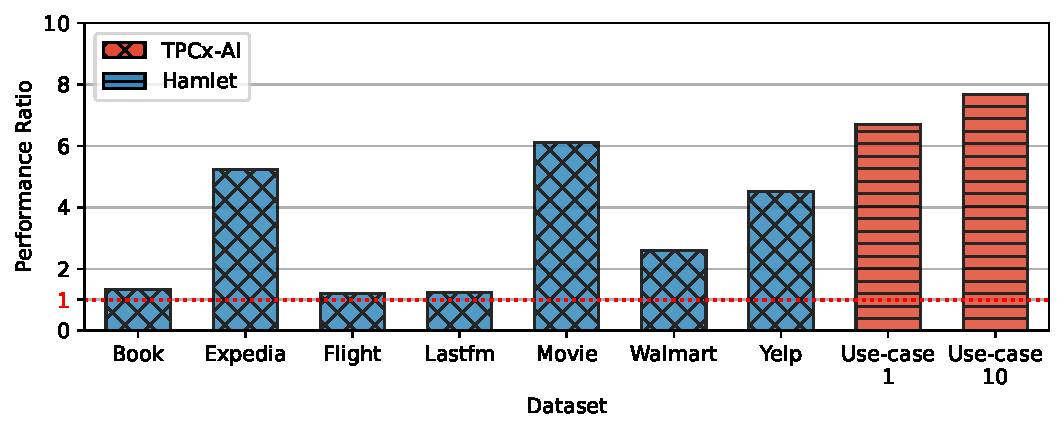
\includegraphics[width=0.9\linewidth]{chapters/05_cost_estimation/figures/real_datasets_speedup.pdf}
    \vspace*{-5mm}
    \caption[Performance ratio with factorization on real datasets]{Average Performance ratio of ML models for positive cases ($\text{Time}_M > \text{Time}_F$), split per tested real dataset and compute type. }
    \label{fig:5-real-perf-ratio}
\end{figure}

The aim of factorized machine learning is to minimize unnecessary operations during model training, thereby enhancing efficiency and speed. The comparative performance of factorization versus materialization on actual datasets is depicted in \autoref{fig:5-real-perf-ratio}. The exploration of factorization proves advantageous; it is observed that in $18\%$ of the instances tested on real datasets, factorization is faster, yielding an average acceleration $5.1\times$. In the most extreme cases, training time is reduced over $20$ seconds, a $27$-fold reduction. Particularly in situations where training is recurrent, such as during hyperparameter tuning or online learning, this efficiency can translate into substantial time savings.

% We group the Data and Model characteristics as they both influence the actual computations being executed. The hardware characteristics influence how these computations are carried out on the hardware and are discussed separately. 

\subsection{Data \& Model Characteristics}
\begin{figure}[ht]
    \centering
    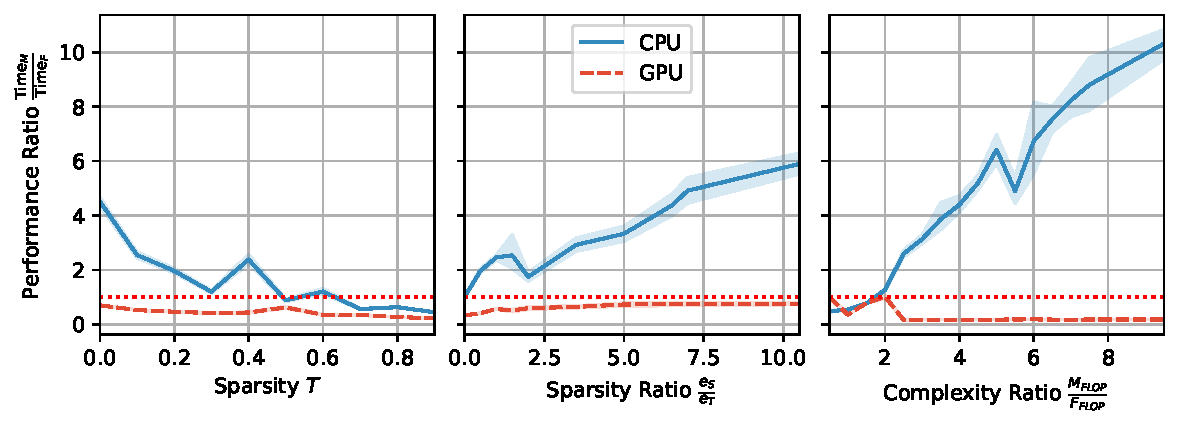
\includegraphics[width=\linewidth]{chapters/05_cost_estimation/figures/motivation_perf_ratio_vs_data_chars.pdf}
    \caption[Performance ratio for various data characteristics]{Performance ratio against various data characteristics. Broken down by compute type (CPU/GPU). $99\%$ confidence interval shown as shaded area. The sparsity ratio is defined as the sparsity of the source tables $S_k, k\in[1,n]$ divided by the sparsity of target table $T$. Sparsity of $S$ is defined as the total non-zero values in the base tables divided by the total number of cells in the base tables, $\frac{\sum_{k=1}^{n} nnz(S_k)}{\sum_{k=1}^{n} r_{S_k} \times c_{S_k}}$. High sparsity ratio means the target table is relatively denser than the source tables.}
    \label{fig:5-complexity-ratio-vs-data-chars}
\end{figure}
We show the influence of different data characteristics on the performance ratio, as depicted in \autoref{fig:5-complexity-ratio-vs-data-chars}. The data reveals a modest inverse relationship between the performance ratio and the sparsity of the target table ($T$). Further analysis, shown in the second column, delves deeper into the connection between performance and sparsity. It indicates that a lower sparsity ratio —meaning ($T$) has a higher count of zero values compared to the base tables ($S_k$)— generally results in factorization being less efficient than materialization. The plots on the far right suggest that a greater complexity ratio ($\frac{FLOP_M}{FLOP_F}$) tends to favor factorization as the optimal training approach. This aligns with the logical premise that factorization is advantageous when it eliminates unnecessary operations.

It is crucial to note that the relationship between these data characteristics and the acceleration provided by factorization becomes less distinct with GPU computations. The reason is that these computations are typically limited by memory capacity rather than processing power. This perspective is examined in detail in \autoref{sec:5-gpu-performance-analysis}, which delves into the metrics gathered during profiling experiments.

\subsection{Hardware Characteristics}
\begin{figure}[ht]
    \centering
    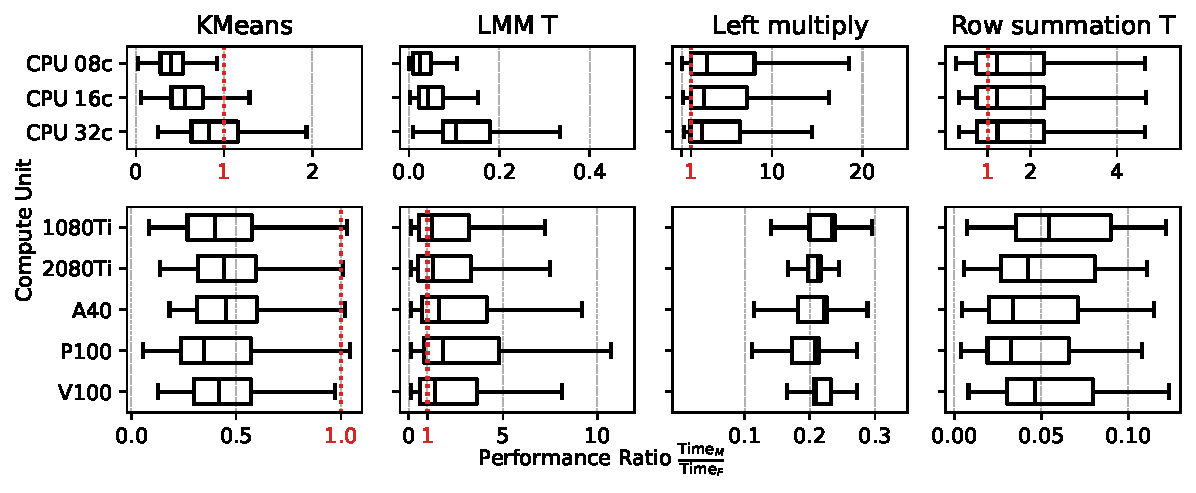
\includegraphics[width=\linewidth]{chapters/05_cost_estimation/figures/motivation_speedup_per_operator_per_gpu.pdf}
    \caption[Performance ratio plotted against hardware]{Performance ratio, of various operators on synthetic data, against hardware. The performance ratio is shown to be affected by hardware choice.}
    \label{fig:5-gpu-characteristics}
\end{figure}
The hardware used for computation not only affects a program's runtime, but also influences the F/M trade-off. Different processing units (i.e., CPU or GPU type) have unique thresholds at which factorization becomes more advantageous than materialization. This phenomenon is illustrated in \autoref{fig:5-gpu-characteristics}. The impact on the performance ratio varies with the hardware and the specific operation performed. For example, the average performance ratio for transposed Left Matrix Multiplication on the P100 GPU is $3.03\pm2.70$, in contrast to a marginally lower $2.32\pm2.21$. On the contrary, for left (scalar) multiplication, the V100 GPU exhibits a higher performance ratio of $0.21\pm0.04$, compared to the P100 $0.19\pm0.05$.

\begin{table}[ht]
    \centering
    % LTeX: enabled=false
\begin{tabular}{lrrrr}
\toprule
Compute Unit & Mean & Std. Dev. & Count & \% with Speedup \\
\midrule\midrule
CPU 08c & 1.27 & 0.25 & 172 & 1.78\% \\
CPU 16c & 1.32 & 0.34 & 579 & 5.99\% \\
CPU 32c & 1.48 & 0.46 & 2873 & 29.74\% \\
1080Ti & 2.27 & 1.60 & 432 & 4.47\% \\
2080Ti & 1.87 & 1.09 & 425 & 4.40\% \\
A40 & 2.00 & 1.20 & 392 & 4.06\% \\
P100 & 2.52 & 1.84 & 461 & 4.77\% \\
V100 & 1.95 & 1.13 & 404 & 4.18\% \\
\bottomrule
\end{tabular}

    \caption[Performance ratio of ML models for cases where factorization has positive impact.]{Mean performance ratio of ML models for cases where factorization is preferred over Materialization (speedup > 1). This shows hardware choice is a large factor in when to choose factorization over Materialization.}
    \label{tab:5-speedup-per-gpu}
\end{table}

In instances where factorization is favored over materialization (when $\text{Time}_M > \text{Time}_F$), the performance varies between different GPUs. Both the average performance ratio and the number of instances where factorization outperforms materialization differ, as indicated in \autoref{tab:5-speedup-per-gpu}. This variation underscores the importance of hardware selection in the factorization versus materialization decision. However, the variation among GPU models is less pronounced than the disparity between CPUs and GPUs. Consequently, it may be more beneficial to consider the type of computation —CPU or GPU— as an independent variable in the cost models rather than focusing on specific GPU models.

When comparing the performance ratio against the complexity ratio for different hardware settings, an interesting pattern emerges. As outlined in \autoref{sec:3-cost-estimation-for-factorized-ml}, the complexity ratio is the ratio of the number of floating-point operations (FLOPs) needed for the factorized case over the materialized case. According to previous research, a higher complexity ratio typically indicates that factorization is more advantageous. However, our experiments reveal that while this is generally true for CPU operations, it does not always apply to GPU computations. This pattern is illustrated in \autoref{fig:5-complexity-ratio-vs-performance-ratio}, and the reasons behind it are explored further in the following section.

\begin{figure}[ht]
    \centering
    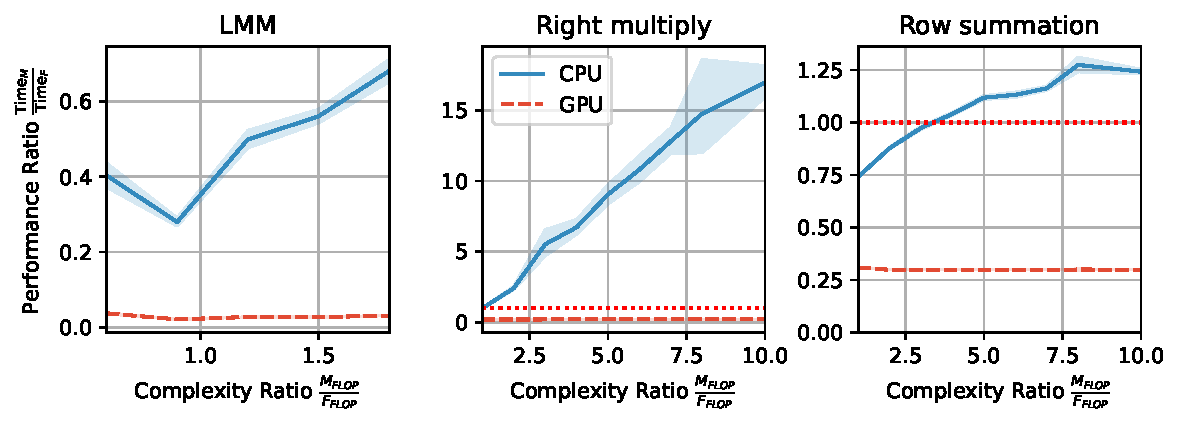
\includegraphics[width=\linewidth]{chapters/05_cost_estimation/figures/motivation_speedup_complexity_ratio.pdf}
    \caption[Performance ratio plotted against complexity ratio]{Performance ratio, of various operators on synthetic data, against complexity ratio, broken down by CPU and GPU. 95\% Confidence interval shown as shaded area. Where a lot of operators show clear correlation between the complexity ratio and the performance ratio on CPU, this is not the case for GPU.}
    \label{fig:5-complexity-ratio-vs-performance-ratio}
\end{figure}


\section{GPU Performance Analysis}
\label{sec:5-gpu-performance-analysis}
An essential preliminary step in creating a precise cost model is understanding the performance attributes of the scenarios under examination. This section analyzes the profiling metrics collected during the experiments to understand the influence of hardware selection on the factorization versus materialization trade-off. The first analysis involves comparing the memory cost and the math cost in the profiled scenarios. According to NVIDIA, an effective method to predict the execution time of a GPU program is to calculate $max(T_{mem}, T_{math})$. In this formula $T_{mem}$ is the time required to transfer data to and from the GPU memory, while $T_{math}$ denotes the time needed for actual computations. This approach is in line with the inherently parallel architecture of GPUs. Should the data transfer to the GPU prove insufficiently fast, the GPU's Streaming Multiprocessors will remain idle, awaiting data. This indicates a memory-bound program. Conversely, if $T_{math} > T_{mem}$, the program is deemed compute-bound. This section elaborates which scenario applies to our experiments and details how this knowledge can be harnessed to estimate the runtime for machine learning training scenarios.

\begin{figure}[ht]
    \centering
    \begin{minipage}{0.50\textwidth}
        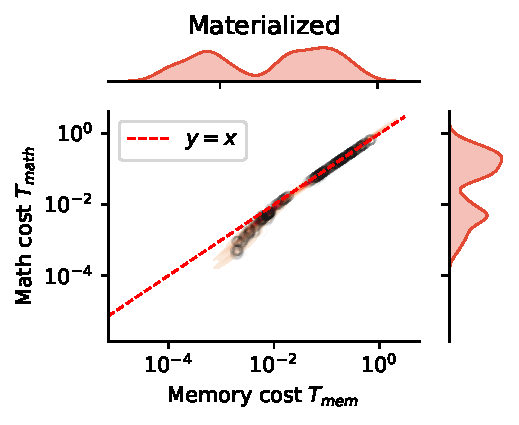
\includegraphics[width=\linewidth]{chapters/05_cost_estimation/figures/profiling-mem-vs-compute-materialized.pdf}
    \end{minipage}\hfill
    \begin{minipage}{0.50\textwidth}
        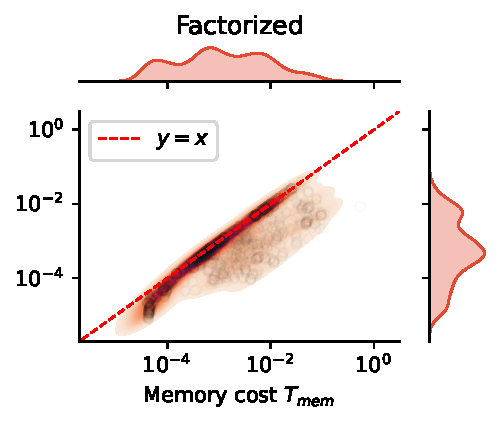
\includegraphics[width=\linewidth]{chapters/05_cost_estimation/figures/profiling-mem-vs-compute-factorized.pdf}
    \end{minipage}
    \caption[Memory cost vs math cost of profiled scenarios]{Memory cost ($T_{mem}$) vs compute cost ($T_{math}$) of profiled scenarios. The memory cost is computed as the total number of bytes read and written to memory divided by the measured average memory bandwidth. The math cost is the number of cycles the Streaming Multiprocessors were active divided by the measured average SM frequency.}
    \label{fig:5-profiling-mem-vs-compute}
\end{figure}

\autoref{fig:5-profiling-mem-vs-compute} shows the relationship between memory time $T_{mem}$ and computation time $T_{math}$, revealing a strong correlation ($\rho = 0.99$). The data predominantly shows that the memory cost exceeds the computational cost, as most points lie below the $y=x$ line, indicating that the operations are memory-bound. This observation suggests that memory cost prediction should be prioritized in our cost estimation efforts. A notable distinction between factorization and materialization emerges when examining their correlation values; materialized cases exhibit a correlation of $\rho = 0.99$, while factorized cases show a significantly lower correlation of $\rho = 0.40$. This discrepancy arises because materialization typically involves handling a single matrix, or two in the case of matrix multiplication. On the contrary, the factorized case on the normalized matrix involves multiple matrices ($S_k,I_k,M_k, k \in \{1 \ldots n\}$), each contributing to different computations. Although this diversity lowers both the memory and the computation costs on average, it also results in a deviation from the $T_{mem} = T_{math}$ equilibrium, due to the sequential execution of computations on these matrices within the GPU.

\begin{figure}
    \centering
    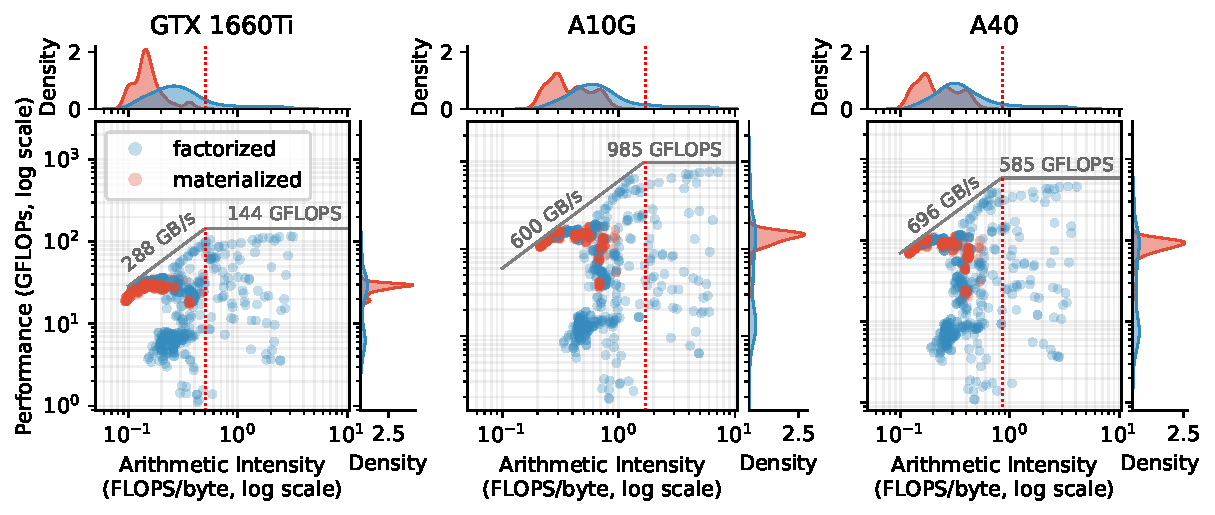
\includegraphics[width=\linewidth]{chapters/05_cost_estimation/figures/roofline-plot.pdf}
    \caption[Roofline chart comparing F/M, per GPU]{Roofline chart showing where the performance of the GPUs lies in the memory-bound vs compute-bound spectrum. The subplots on top and right side of each figure show the distribution along the performance (GFLOPs) and operational intensity (FLOPS/byte) axes. Similar GPU types have similar distributions.}
    \label{fig:5-roofline-plot}
\end{figure}

\subsubsection*{Roofline Model}
More insights into the efficiency of the tested scenarios, and the differences between factorization and materialization, and GPU types, can be gained by using a roofline model. It is a “model that offers insight insights \ldots on improving parallel software and hardware for floating point computations” \cite{roofline}. The model delineates whether an operation is constrained by memory or computation. On the x-axis, it plots the arithmetic intensity of a program (in our context this refers to an operator applied to a dataset), measured in FLOPs per byte. The y-axis represents the achievable performance in GFLOPS. The roofline itself (illustrated in gray) signifies the performance limit for a particular GPU, derived from its maximum memory bandwidth and computational capacity in FLOPs per second. The intersection point, known as the ``ridge point,'' indicates the minimum arithmetic intensity required to fully leverage the computational capabilities of the GPU. By plotting programs this chart one can infer whether a program is memory-bound (to the left of the ridge point) or compute-bound (to the right of the ridge point). This analysis is crucial because it highlights potential optimization possibilities by pinpointing performance bottlenecks.

% The roofline charts for the performed profiling experiments are shown in \autoref{fig:5-roofline-plot}. These charts confirm that almost all scenarios are memory-bound. But, the interesting observation from this plot is the impact of GPU type, and the difference between factorization and materialization. The differences between GPUs are most obvious in the right distribution plots. The A10G and A40 are much more powerful GPUs. On the GTX1660Ti most scenarios reach a low compute performance as they hit the memory bound. The A10G and A40, however, have a much higher memory bandwidth. Thus, the scenarios reach a higher average performance. The gap these plots show between factorization and materialization gives more valuable insights. 

% The materialized operators have lower arithmetic complexity than their factorized equivalents (shown in the top density plots). This means that, on average, the factorized operators are less memory-bound, and thus can utilize a larger part of the GPUs compute capacity. However, the factorized operators show a much larger variance in attained performance (right density plots) due to the fact that the operations on different parts of the normalized matrix are not parallelized. These operators can likely be optimized, so they can take advantage of the GPUs compute capacity more efficiently.

The roofline charts depicted in \autoref{fig:5-roofline-plot} validate that most scenarios are constrained by memory. However, what stands out is the impact of the GPU type on performance, as well as the contrast between factorization and materialization. The difference among GPU models is particularly evident in the distribution plots to the right of each subplot. High-performance GPUs such as the A10G and A40 demonstrate a superior memory bandwidth compared to the GTX1660Ti, which often reaches a plateau in performance due to memory bandwidth limitations. Consequently, scenarios involving the A10G and A40 achieve a higher average performance.

The divergence between factorization and materialization highlighted in these graphs is insightful. Materialized operators exhibit lower arithmetic complexity than their factorized counterparts, as indicated in the top density plots. This suggests that factorized operators, on average, are less constrained by memory, allowing them to better leverage the computational resources of the GPU. However, the significant variability in performance achieved by factorized operators, as shown in the right density plots, is due to the sequential execution of operations on different matrix segments. There is potential for optimization here, which could allow these operators to more effectively utilize the GPU’s computational power.

\begin{figure}[ht]
    \centering
    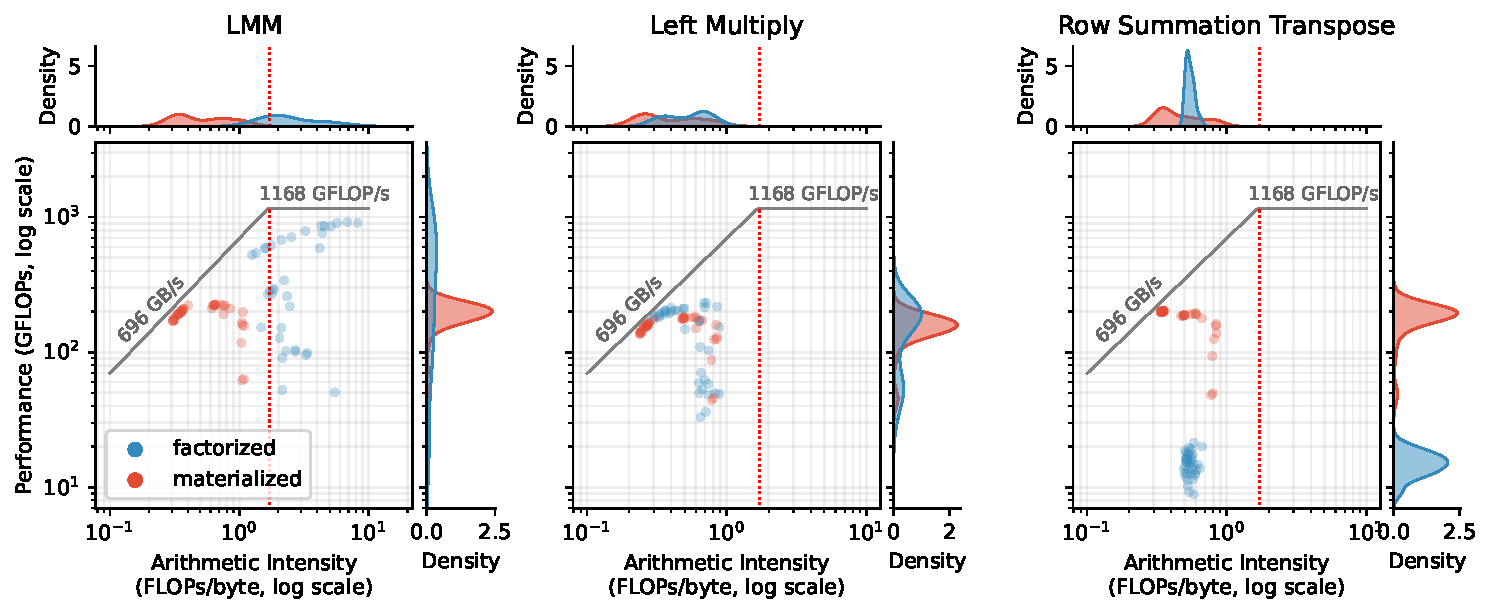
\includegraphics[width=\linewidth]{chapters/05_cost_estimation/figures/roofline-operators.pdf}
    \caption[Roofline chart per operator]{Roofline chart comparing factorization and materialization for Left Matrix Multiplication, Left Scalar Multiplication and Row Summation Transpose. Metrics from NVIDIA A40.}
    \label{fig:5-roofline-operators}
\end{figure}

A roofline chart for a selection of operators is shown in \autoref{fig:5-roofline-operators}. This breakdown per operator further shows the differences between factorization and materialization. Compared to the materialized case, the factorized case of Left Matrix Multiplication shows extremely large variance in performance, which is in line with the use of the normalized matrix explained previously. Although overall, using factorization seems beneficial for LMM when looking at these profiling metrics (values move to the top and right, indicating higher saturation of the available resources). For Left Scalar Multiplication the gap between F and M is much smaller, which is logical as the factorized case only multiplies the Source matrices with the scalar, which is a simpler operation than the one needed for LMM. The right-most plot shows this limitation even more clearly, showing significantly less utilization of the GPU capabilities than the materialized case for Transpose Row Summation. The complete set of roofline plots broken down per operator can be found in \autoref{appendix:analysis-additional-figures}.

The roofline chart in \autoref{fig:5-roofline-operators} provides a detailed comparison of different operators, highlighting the distinctions between factorization and materialization. For Left Matrix Multiplication (LMM), the factorized approach exhibits large variance in performance, aligning with the previously mentioned use of a normalized matrix. Despite this variance, factorization generally appears to be advantageous for LMM, as indicated by the profiling metrics that suggest a more complete utilization of GPU resources. In contrast, the difference in performance between factorized and materialized cases for Left Scalar Multiplication is less pronounced. This is expected, since the factorized operation is simpler and involves only the multiplication of source matrices by a scalar. The right-most plot reveals a clear underutilization of GPU capabilities for Transpose Row Summation in the factorized form, compared to the materialized one. This suggests that while factorization can be beneficial for certain operations, it may not always be the most efficient use of GPU resources. For a comprehensive view of all operators, the full suite of roofline plots is available in \autoref{appendix:analysis-additional-figures}, providing insight into the performance dynamics of each operator.

\section{Feature Engineering}
\label{sec:5-feature-engineering}
We proceed to construct a well-suited dataset for training our cost models. By building on the foundational work that has revealed the relations between speedup and various data and hardware characteristics in \autoref{sec:5-motivation}, and by incorporating the insights from our profiling analysis we enrich and process the dataset.

This dataset, gathered through our comprehensive experiments, has a sample for each unique scenario, with the runtime and the attributes of dataset, the operator type, the model form (factorized/materialized), and the hardware configuration. The following section outlines the preprocessing and augmentation of this dataset with additional features. The enrichment process is designed to capture the complex interactions and patterns we have observed. The features are carefully crafted to enhance the estimators' ability to make predictions about when to use factorization or materialization. The complete set of features is detailed in \autoref{appendix:features}, with a focused discussion on a select subset presented in \autoref{tab:5-feature-subset}.

\subsection{Preprocessing Profiling Metrics}
\begin{figure}[ht]
    \centering
    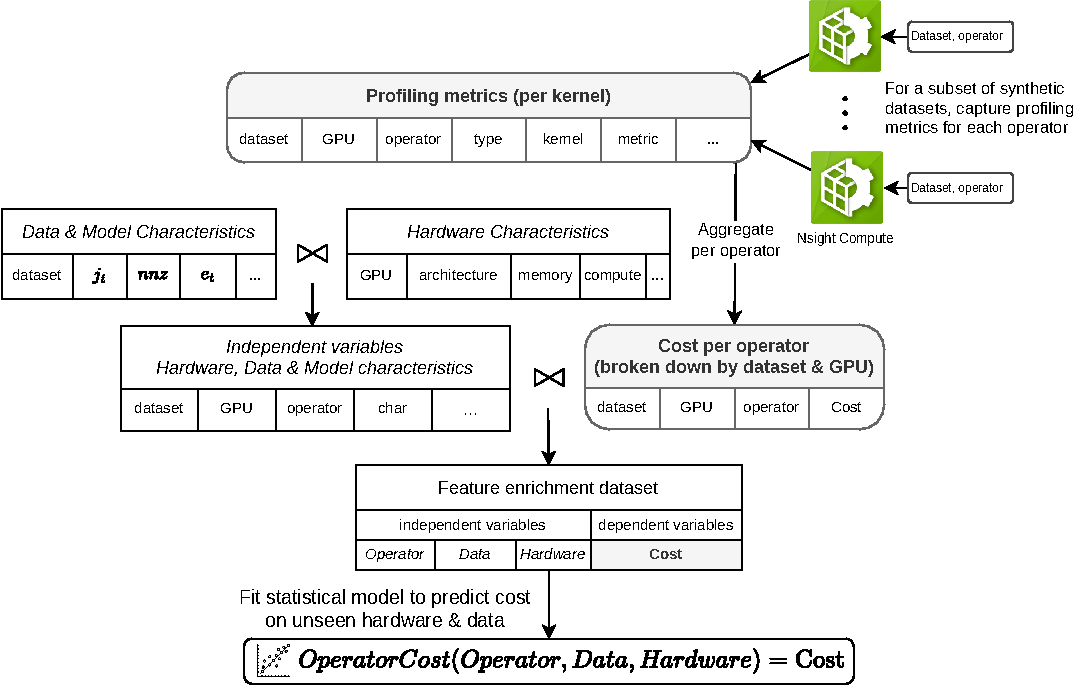
\includegraphics[width=\linewidth]{chapters/05_cost_estimation/figures/feature-engineering.pdf}
    \caption[Feature enrichment workflow]{Workflow of enriching the collected data with additional features from the profiling experiments. Items related to these profiling experiments are \textbf{bolded}, while the features from the data, model \& hardware characteristics are \textit{italicized}. Description for the aggregation process (“1”) is in \autoref{sec:5-feature-engineering}.}
    \label{fig:5-feature-enrichment}
\end{figure}
The feature engineering process begins with the integration of the profiling metrics into the dataset. This process, however, presents two significant challenges. The first challenge arises from the fact that these metrics are gathered at the kernel level, while our focus is on operator performance. To address this, we aggregate kernel-level metrics to reflect the performance of the entire scenario. The second challenge is the incomplete coverage of metrics, as they were collected for a subset of scenarios. The strategy for overcoming these obstacles is depicted in \autoref{fig:5-feature-enrichment} and is further detailed below.

The procedure for aggregating kernel-level metrics to operator-level metrics is outlined as follows, and is also depicted in \autoref{fig:5-feature-enrichment}, marked by the “1”. For each scenario, we compute the sum of the metrics that are totals, i.e., the metrics with units of nanoseconds, bytes, or cycles (refer to \autoref{tab:4-profiling-metrics} for applicable metrics). The remaining metrics are either percentages or measures per second. For these metrics, we calculate the weighted average, where the weight is the kernel’s runtime. This ensures that the metrics accurately represent the total runtime of the scenario. This procedure yields precise operator-level metrics for each scenario.

\begin{table}[ht]
    \centering
    \begin{tabular}{p{0.19\linewidth}p{0.37\linewidth}>{\footnotesize}p{0.35\linewidth}}
        \toprule
        Feature                                   & Formula                                                                                                 & Description                                                                                                                                       \\
        \midrule\midrule
        \texttt{dram\_bytes\_sum}                 & $\texttt{dram\_bytes\_read\_sum} + \texttt{dram\_bytes\_write\_sum}$                                    & Total number of bytes read and written to DRAM.                                                                                                   \\
        $T_{mem}$                                 & $\frac{\texttt{dram\_bytes\_sum}}{\texttt{memory\_throughput\_byte\_weighted\_mean}}$                   & Total memory bytes divided by the achieved memory throughput. Gives the cost of the involved memory operators in seconds.                         \\
        $T_{math}$                                & $\frac{\texttt{sm\_active\_cycles\_sum}}{\texttt{sm\_frequency\_weighted\_mean}}$                       & Total active cycles divided by the achieved frequency of the Streaming Multiprocessors. Gives the cost of the involved math operators in seconds. \\
        \texttt{FLOPs}                            & $\frac{\texttt{compute\_throughput\_weighted\_mean}}{100} \times \text{\small{gpu\_processing\_power}}$ & Total number of FLOPs executed in the scenario. Processing power is for double precision.                                                         \\
        \texttt{arithmetic\_-} \texttt{intensity} & $\frac{\texttt{FLOPs} \times \texttt{duration}}{\texttt{dram\_bytes\_sum}}$                             & The number of FLOPs executed per byte read or written to memory.                                                                                  \\

        \bottomrule
    \end{tabular}
    \caption[Derived features]{Overview of features computed from the profiling metrics. Features starting with "gpu" are constants for the specific GPU used.}
    \label{tab:5-derived-features}
\end{table}

The second issue pertains to the fact that metrics are not collected for all scenarios. This is addressed by fitting a statistical model to the collected metrics and employing this model to predict the missing metrics. The model, denoted as $OperatorCost$ in \autoref{fig:5-feature-enrichment}, is an ensemble of linear regressors. It uses aggregated metrics, hardware characteristics, and data characteristics as features, with memory cost $T_{mem}$ as the target variable. Each combination of operator and training type (F/M) has its own linear regression model.
To enhance the model, we engineer an additional set of features derived from the metrics collected, as shown in \autoref{tab:5-derived-features}.
The model is trained on a subset of the metrics collected and tested on the remaining metrics. Subsequently, the model is used to predict the missing metrics. This process is crucial to ensure that we have metrics for all scenarios, as the cost models require a complete dataset for training. The true versus predicted values of this estimator are depicted in \autoref{fig:5-analytical-regressor-fit}.

\begin{figure}[ht]
    \centering
    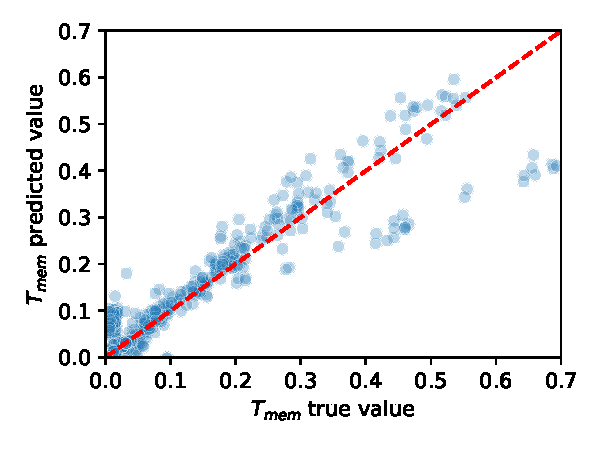
\includegraphics[width=0.5\linewidth]{chapters/05_cost_estimation/figures/analytical-regressor-fit.pdf}
    \caption[Analytical estimator memory cost prediction vs. true values]{True $T_{mem}$ vs. predicted $T_{mem}$ for the analytical estimator's $OperatorCost$ function. Tested on samples not used for training. MSE: $0.0295$.}
    \label{fig:5-analytical-regressor-fit}
\end{figure}

\subsection{Model-level Math and Memory cost}
\label{subsec:5-model-level-cost}
In this section, we describe the process of calculating the memory and mathematical costs for each scenario. Contrary to the previous section, which estimated the memory cost as perceived by the GPU, we now compute the theoretical costs. Memory cost is determined by dividing the total number of bytes read and written to memory by memory throughput. The mathematical cost is computed as the total number of FLOPs required for a computation. These definitions align with those used in the profiling experiments. However, in this context, we derive them from the available data and model characteristics, rather than predicting them using a regressor, as was explained in the preceding section.

The complexity of an operator or model, as previously detailed, is equal to the mathematical costs and is determined by examining the algorithms and summing the computations performed. This process takes into account various data characteristics, such as the number of non-zero items and dataset sizes. For memory costs, a similar approach is employed, but we sum the number of bytes read and written to memory. For each Machine Learning (ML) model, we incorporate both the total summed costs and the costs per involved operator as features. This results in a multitude of additional features that can be utilized to train the cost models.

A subset of these features is presented in \autoref{tab:5-feature-subset}. The complete set of features is displayed in \autoref{appendix:features}. These features are used to train the cost models, as will be detailed in the subsequent section.

\begin{table}[ht]
    % LTeX: enabled=false
\begin{tabular}{llll}
\toprule
Dimension & Feature & Symbol & Formula \\
\midrule\midrule
\multirow[t]{5}{*}{Data} & Dataset size (rows, columns) & $r_T, c_T$ &  \\

 & Sparsity & $e_T$ & $\frac{nnz(T)}{r_T\times c_T}$ \\

 & Sparsity ratio &  & $\frac{e_T}{e_S}$ \\

 & Tuple ratio & $\tau$ & $\frac{\sum_{k=1}^p d_k}{d_S}$ \\

 & \# Base tables & $n$ &  \\
 
\multirow[t]{2}{*}{Data \& Model} & Complexity ratio &  & $\frac{FLOP_M}{FLOP_F}$ \\

 & Memory ratio &  & $\frac{\text{bytes}_M}{\text{bytes}_F}$ \\
 
\multirow[t]{2}{*}{Hardware} & Compute type &  &  \\

 & GPU memory bandwidth &  &  \\
 
\multirow[t]{2}{*}{Model} & Operator &  &  \\

 & \# Iterations & $iter$ &  \\
 
\multirow[t]{3}{*}{\textbf{Dependent}} & Execution Time & $\text{Time}_M$, $\text{Time}_F$ &  \\

 & Performance ratio &  & $\frac{\text{Time}_M}{\text{Time}_F}$ \\

 & Time saved &  & $\text{Time}_M - \text{Time}_F$ \\
 
\bottomrule
\end{tabular}

    \caption[Feature table]{Table showing a subset of the base, and derived/engineered features used for training the cost models}
    \label{tab:5-feature-subset}
\end{table}

\section{Cost Models}
\label{sec:5-cost-models}
This section details the process of developing four different types of cost estimators, each capable of choosing when to favor factorization over materialization. These estimators are constructed using the enriched dataset, as described in the preceding section. We start with an introduction of the metrics used to evaluate cost model performance (\autoref{sec:5-metrics}), followed by the estimators themselves. The first estimator, designed to be as interpretable as possible, is an analytical estimator (\autoref{subsec:5-analytical}). Next, we fit a range of linear regressors to the dataset to create an estimator (\autoref{subsec:5-linear-regression}). The third estimator is a tree-boosting model, employed to demonstrate the performance of a more intricate model (\autoref{subsec:5-xgboost}). The final estimator is a hybrid model, which merges the linear regression and tree-boosting estimators to yield a more precise model.

\subsection{Problem Modelling and Assessing Performance}
\label{sec:5-metrics}
The decision whether to opt for factorization or materialization is a binary classification challenge. However, it is more important to accurately predict scenarios that lead to greater time saved. As a result, we use regression models over classification models. This approach enables us to define the decision boundary, allowing greater flexibility in prioritizing scenarios with larger performance benefits.

\subsubsection{Metrics to Assess Cost Model Performance}
To evaluate the performance of the cost models, we employ a set of metrics that provide insight into the accuracy and efficiency of the models. Previous work \cite{schijndel_cost_estimation,orion_learning_gen_lin_models,MorpheusFI} uses accuracy and performance ratio values to reason about the effectiveness of their cost estimation techniques. However, as the dataset is imbalanced, and a majority of scenarios favor materialization, accuracy is not a suitable metric. The performance ratio also has limitations, as one loses a lot of information when averaging the ratio of multiple scenarios into a single value, as it does not capture how much time was saved, which is the more informative metric when assessing cost model performance for a set of scenarios.

Consequently, we introduce a new metric, It is the difference between the sum of materialized times and the sum of factorized times, for those cases where the cost models predict factorization to be faster. This gives a more realistic view of how useful the estimator would be in real-world settings, as the cases where the cost model predicts materialization to be faster are less relevant. Such a case will not result in a time loss compared to the normal, materialized execution. However, because we want to reason about whether the models have sufficient performance, we also include the maximum possible time saved as a benchmark. As scenarios were the time savings are larger are more important, we weigh the performance ratio by the time saved. This gives a more nuanced view of the relative performance gains. The last metric, which is used to verify generalizability in \autoref{subsec:6-generalizability}, is the utility of an estimator: the fraction of time saved when using this estimator, relative to the maximum time saved. These metrics are summarized in \autoref{tab:metrics}.

\begin{table}[ht]
    \centering
    \renewcommand{\arraystretch}{1.5} % Adjust the row separation here
    \resizebox{\textwidth}{!}{%
        \begin{tabular}{p{0.2\linewidth}p{0.35\linewidth}p{0.4\linewidth}}
            \toprule
            Metric                      & Formula                                                                                       & Description                                                                               \\
            \midrule\midrule
            Time Saved                  & $\sum\text{Time}_M - \sum \text{Time}_F$ where Factorization is predicted to be faster        & The sum of the time saved for all positively predicted scenarios.                         \\
            Maximum Possible Time Saved & $\sum \text{Time}_M - \sum \text{Time}_F$ where Factorization is faster                       & The maximum possible time that could be saved.                                            \\
            Weighted Performance Ratio  & $\frac{\sum \text{Time}_M}{\sum \text{Time}_F}$ where Factorization is predicted to be faster & The ratio of the total materialization time to the total factorization time.              \\
            Utility                     & $U = \frac{\text{Time Saved}}{\text{Max. Time Saved}}$                                        & The fraction of time saved when using this estimator, relative to the maximum time saved. \\
            \bottomrule
        \end{tabular}}
    \caption{Metrics to Assess Cost Model Performance}
    \label{tab:metrics}
\end{table}


\subsection{Analytical}
\label{subsec:5-analytical}
\begin{figure}[ht]
    \centering
    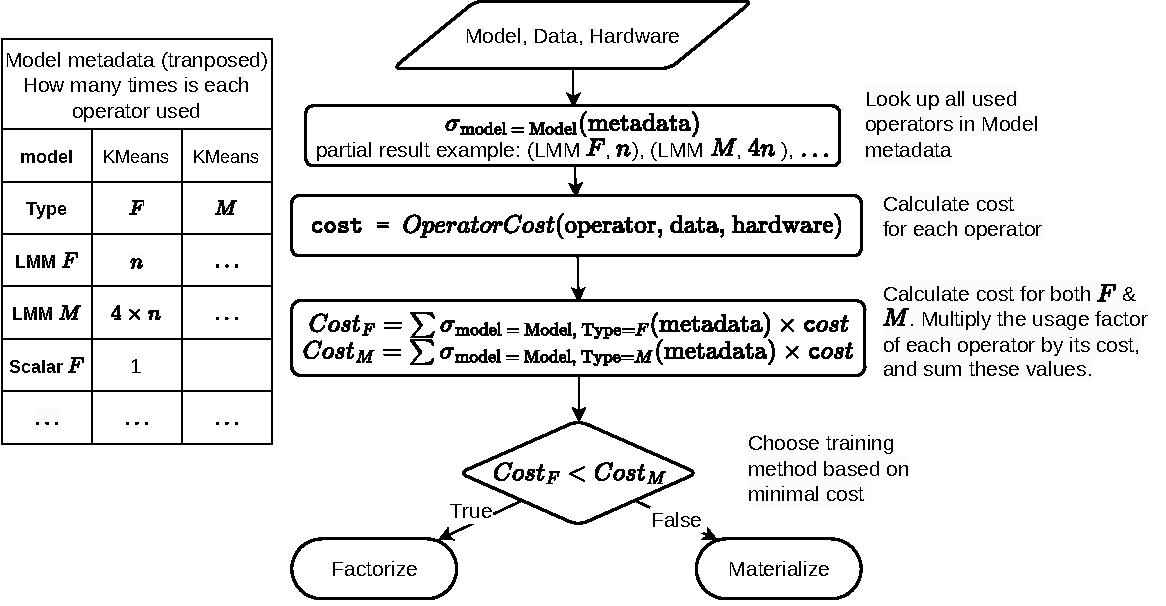
\includegraphics[width=\linewidth]{chapters/05_cost_estimation/figures/analytical-architecture.pdf}
    \caption[Analytical Estimator Architecture]{Architecture of the Analytical Estimator. Shows the control flow of inputs to a final decision on whether to use factorization or materialization. $OperatorCost$ is the function as defined in \autoref{fig:5-feature-enrichment}.}
    \label{fig:5-analytical-architecture}
\end{figure}

As demonstrated in \autoref{sec:5-gpu-performance-analysis}, the runtime of the evaluated Machine Learning scenarios is primarily determined by the time required to read and write to memory. Consequently, to generate an accurate prediction of the execution time of a scenario, we can use memory cost as a proxy measure, an approach adopted by this analytical estimator.

\subsubsection*{ANLY.1 Profiling Metrics Based Estimator}
The workflow for computing the factorized and materialized memory cost is shown in \autoref{fig:5-analytical-architecture}. We first collect the operators used for the model under test. We then use a regressor fit to the collected profiling metrics (as shown in \autoref{fig:5-feature-enrichment}) to predict the factorized and materialized operators' memory cost. This step is necessary as we do not have profiling metrics for the scenarios we are testing. Last, the costs for each training type are summed, and choose the scenario with the lowest predicted runtime.

The procedure to calculate the factorized and materialized memory cost is depicted in \autoref{fig:5-analytical-architecture}. First, we gather the operators used in the model under evaluation. Next, we employ a regression model, fitted to the collected profiling metrics (as illustrated in \autoref{fig:5-feature-enrichment}), to predict the memory cost of the factorized and materialized operators. This step is indispensable, as we lack profiling metrics for the scenarios under test. Finally, we sum the costs for each training type and select the scenario with the lowest predicted runtime.

A significant limitation of this estimator is its dependence on a pretrained regressor to predict the memory cost. This regressor is trained on a subset of the collected metrics and is utilized to predict the missing metrics. The regressor we employ is fitted to a subset of factorized and materialized operator scenarios, making it unsuitable for predicting the cost of operations that deviate from the tested scenarios. The development of an estimator capable of predicting the memory cost for all scenarios is a complex undertaking and is left for future work.

\subsubsection*{ANLY.2 Model-level Memory Cost Analysis Based Estimator}
By inspecting the operations performed during ML model training, we can calculate the number of bytes read and written during computation. This is achieved by calculating the number of bytes read and written for each operation and summing these values. The memory cost is subsequently determined by dividing the total number of bytes read and written by the GPU’s memory throughput. Compared to ANLY.1, this estimator is more adaptable to new ML models, as it does not require a pretrained regressor to estimate operator cost. However, it does not consider other factors that influence memory cost, such as cache layout and hit rates.

\subsubsection{Analytical Model Evaluation}
Both analytical estimators yield a predicted memory cost for the factorized and materialized cases. To arrive at the final decision, we compute the ratio between the cases and opt for factorization if this ratio ($\frac{M}{F}$) exceeds a certain threshold. This threshold is fine-tuned to minimize the number of false positives while still favoring factorization in instances where it significantly outperforms materialization in terms of time efficiency. For the first analytical estimator (ANLY.1), we set the threshold at $1.7$, and for ANLY.2, we set it at $10.0$. The fact that the model only performs well with such a high ratio of materialized to factorized memory cost indicates that factorization introduces considerable overhead in areas not captured by this simplistic memory estimation.

The results of the evaluation are shown in \autoref{fig:5-analytical-model-evaluation}. Both models perform similarly well. The ANLY.1 model predicts a lot less false positives, but the sum of time lost by these false positives is almost the same as that of the FPs for ANLY.2. Subtracting the time lost for the FPs from the time saved for the true positives, we see that ANLY.2 saves more time than ANLY.1. This is likely due to the fact that ANLY.2 is more conservative in predicting factorization, and thus has a higher threshold for when to choose factorization over materialization. Altogether both models save around 250s of the total 1670s of the validation set. Breaking down the positively predicted cases by compute type we see that a lot of time (147s \& 136s respectively, shown in \autoref{fig:5-model-cpu-gpu}) is lost for false positives of CPU scenarios. So, for GPU scenarios the model is more accurate than for CPU scenarios, which is expected as we only use memory cost as an estimator for runtime. We have shown this to be a valid strategy for GPUs, but for CPUs the runtime is largely dominated by the number of FLOPs executed.

The evaluation results are presented in \autoref{fig:5-analytical-model-evaluation}. Both models, ANLY.1 and ANLY.2, exhibit comparable performance. Although ANLY.1 predicts fewer false positives, the cumulative time lost due to these false positives is nearly identical to that of ANLY.2. By subtracting the time lost due to false positives from the time saved by true positives, it is observed that ANLY.2 saves more time than ANLY.1. This is likely because ANLY.2 adopts a more conservative approach in predicting factorization, thus having a higher threshold for choosing factorization over materialization.

Both models save approximately $250$ seconds of the total $1670$ seconds of the validation set. When we break down the positively predicted cases by compute type, we find that a significant amount of time ($147$ seconds and $136$ seconds respectively, as shown in \autoref{fig:5-model-cpu-gpu}) is lost due to false positives in CPU scenarios. So, these models are more accurate for GPU scenarios than for CPU scenarios, which aligns with our expectation, as we use memory cost as an estimator for runtime. We have demonstrated this to be a valid strategy for GPUs, but for CPUs, the runtime is predominantly determined by the number of Floating Point Operations Per Second (FLOPs) executed.

\begin{figure}[ht]
    \centering
    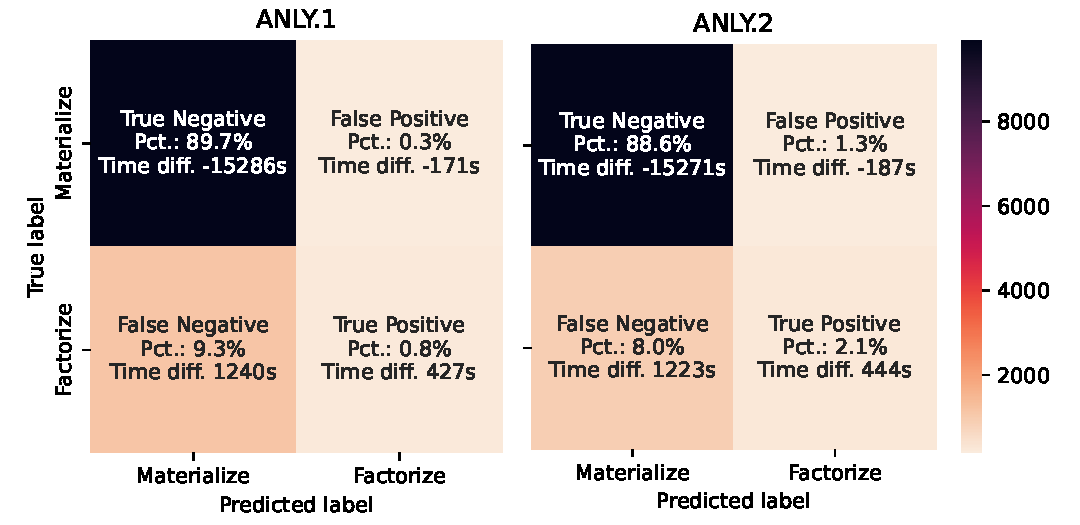
\includegraphics[width=0.9\linewidth]{chapters/05_cost_estimation/figures/analytical-models-compare.pdf}
    \caption[Analytical Model Confusion Matrix]{Confusion matrix of the analytical models' performance on the test set (CPU and GPU on synthetic data). Decision boundaries set at $1.7$ and $10.0$ respectively. Adding time difference of the false positive cases and the true positive cases gives the total time saved by the model. For ANLY.1 this is 256s, for ANLY.2 it is 257s. }
    \label{fig:5-analytical-model-evaluation}
\end{figure}


\subsection{Linear Regression}
\label{subsec:5-linear-regression}
In this section, we delve into the second type of cost estimator, the linear regression estimator. The objective of this estimator is to maintain explainability while delivering superior performance compared to the manually tuned decision rules found in related works. We employ a range of models, all of which fundamentally rely on linear regression. We start with a single regressor and, by partitioning the dataset according to the categorical variables, we eventually arrive at more intricate models comprising ensembles of linear regression models.

The architecture of each of the linear regression models is shown in \autoref{fig:5-linear-regression-architecture}. In short, before training the dataset is split by a number of categorical variables (operator type, hardware type or $F$/$M$), or by filtering a part of the dataset. Each final model is a set of Linear Regression models, each fit to one of the subsets of the training data. For example, for LINR.3 we train two regressors. One on the factorization scenarios and one on the materialization scenarios. During inference, each of the regressors is used to predict the runtime of the scenario under test. The output is the predicted materialized time minus the predicted factorized time. This is done to predict the time saved by choosing factorization over materialization. When a categorical variable is not used to split the dataset, it is used as a feature in the model.

The architecture of each of the linear regression models is depicted in \autoref{fig:5-linear-regression-architecture}. In short, before training, the dataset is partitioned according to several categorical variables (operator type, hardware type, or F/M), or by filtering a portion of the dataset. Each final model comprises a set of Linear Regression models, each fit to a subset of the training data. For example, for LINR.3, we train two regressors: one for the factorization scenarios and the other for the materialization scenarios. During inference, each regressor is used to predict the runtime of the scenario under test. The output is the difference between the predicted materialized time and the predicted factorized time, which is used to estimate the time saved by opting for factorization over materialization. If a categorical variable is not used to split the dataset, it is incorporated as a feature in the model.

\begin{figure}[ht]
    \centering
    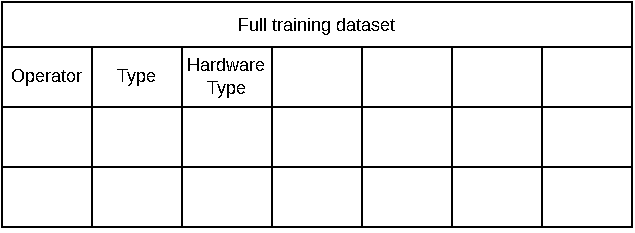
\includegraphics[width=\linewidth]{chapters/05_cost_estimation/figures/statistical-architecture.pdf}
    \caption[Linear Regression Estimator Architecture]{Architecture of the Linear Regression Estimators. Shows how the data, and estimators, are split for each model. The final split-level belonging to each respective model is colored in the same color. For LINR.5 we show the linear regression ensemble fit to the data. For clarity, we leave this out for the other models. Each box represents a regression model, the same-colored boxes, connected via dotted lines, are combined into an ensemble to end up with the linear regression cost estimators.}
    \label{fig:5-linear-regression-architecture}
\end{figure}

\subsubsection*{LINR.1 Linear Regressor Fit to Full Training Set}
The first linear regressor is trained on the complete training set, which includes all operators. The rationale behind this approach is the probable existence of a correlation between the performance of individual operators and the performance of the models in which they are used. By training the regressor on the entire set of operators, we strive to capture these correlations and leverage them to enhance accuracy. This model predicts the time conserved by opting for factorization over materialization.

\subsubsection*{LINR.2 Linear Regressor Fit to Model Runtimes}
The second linear regressor is trained only on the runtimes of the models, the individual operators are left out of the training set. This model helps determine whether the inclusion of operators contributes to utility. Similarly to LINR.1, this model forecasts the time conserved by opting for factorization over materialization.

\subsubsection*{LINR.3 Separate Regressors for F and M}
This model is a composite of two linear regressors, one for factorization and another for materialization. By training distinct regressors for factorization and materialization, we aim to more explicitly capture the correlations between independent variables and runtime than the preceding models. Each internal regressor predicts the runtime of the scenario under test, and the final prediction is the faster predicted scenario.

\subsubsection*{LINR.4 Separate Regressors for each Model Type}
Similar to LINR.3, this estimator is also a composite of multiple internal regressors. However, instead of having a single regressor for each factorization and materialization, we have a distinct regressor for each model type. This is done to capture the differences in the correlations between independent variables and runtime for different model types. Like the first two models, this model forecasts the time saved by choosing factorization over materialization (by predicting whether time is conserved by choosing F).

\subsubsection*{LINR.5 Separate Regressors for CPU and GPU}
In previous sections, we have shown that the choice of hardware plays a significant role in the trade-off we investigate. Therefore, it is likely that there are differences in the correlations between independent variables and runtime between CPU and GPU. A singular linear regression model is probably incapable of capturing these differences. Consequently, we test the performance of a set of estimators, one which is only fit to CPU scenarios, and another which is only fit to GPU scenarios.

\subsubsection*{LINR.6 Separate Regressors for F, M and Model Type}
The next version of the linear regression model we create is a composite of LINR.4 and LINR.3. By training separate regressors for every combination of factorization, materialization, and model type, we enable the models to more freely capture differences between groups.

\subsubsection*{LINR.7 Separate Regressors For Each Combination of Categories}
The final, most granular, ensemble is one that has a distinct regressor for each combination of factorization, materialization, model type, and hardware. This is done to capture the differences in the correlations between independent variables and runtime for each combination of the dimensions.


\subsubsection{Linear Regression Model Evaluation}
\begin{figure}[ht]
    \centering
    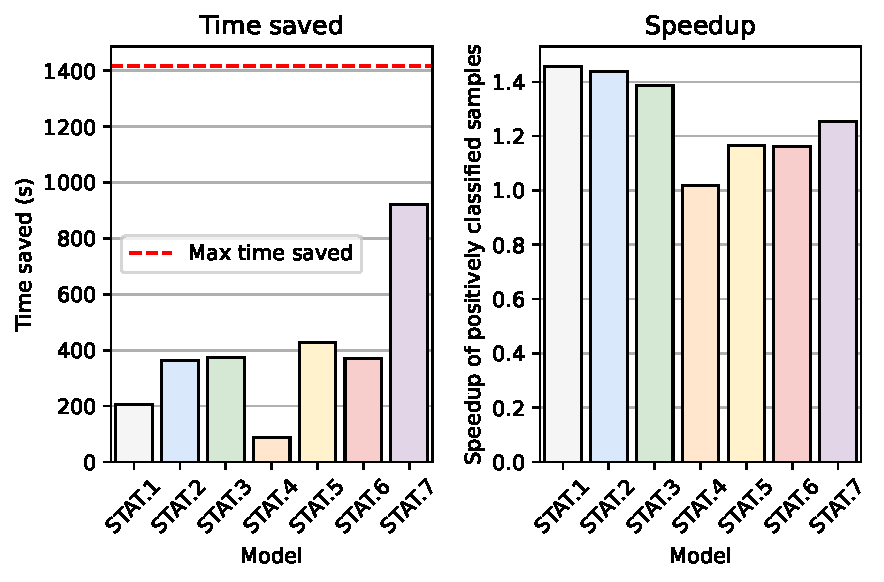
\includegraphics[width=0.75\linewidth]{chapters/05_cost_estimation/figures/stat-models-compare.pdf}
    \caption[Linear Regression Model Evaluation]{Evaluation of the linear regression models on the validation set (synthetic data, only models). The plots show statistics of those scenarios where the estimator predicts factorization to be faster. The plot on the left shows $\sum \text{Time}_M - \sum \text{Time}_F$, the total time saved across positively predicted scenarios. The right plots show $\frac{\text{Time}_M}{\text{Time}_F}$ highlighting that conservative estimators can result in high performance ratio's with a low amount of time saved, for example LINR.7.}
    \label{fig:5-linear-regression-model-evaluation}
\end{figure}

A performance comparison for the linear regression models is shown in \autoref{fig:5-linear-regression-model-evaluation}. We choose to highlight the cases where the model predicts factorization to be faster, and evaluate the saved time in these cases. Overall, estimators that fit more distinct regressors perform better, showing that each of the chosen categorical variables impacts the F/M trade-off.

Models LINR.1 through LINR.3 demonstrate relatively minimal time saved, but the average speedup of positively classified cases is high. This is attributable to these models either producing a substantial number of false negatives, thereby missing out on a significant amount of time saved (LINR.1), or many false positives, which reduces the total time saved (LINR.2 and LINR.3). LINR.4, which is split solely by model type, performs the worst among the estimators, indicating that there is a relationship between the different model types. The LINR.5 and LINR.6 estimators both identify a relatively large fraction of positive samples, albeit at the cost of numerous false positives and negatives. LINR.7, which is the most granular, performs the best on the \textbf{validation} set. This is likely because it can capture the differences in the relationships between independent variables and runtime for each combination of the dimensions. This estimator is the most complex, but also the most accurate, performing $65\%$ as well as a perfect cost model when considering the time saved.

However, when evaluating on the \textbf{test} datasets (visualized in \autoref{fig:5-model-cpu-gpu} for LINR.1 and LINR.5), the performance of the models is considerably lower. This is likely due to the models overfitting to the training data (which contains only synthetic dataset scenarios). Only the LINR.1 and LINR.5 models perform relatively well, which can be explained by the fact that they do not use extensive partitioning of the training data, thereby preventing the regression from fitting to the training data. To address this overfitting, we choose to evaluate the performance of a more complex model.

% However, when evaluating on the test datasets, the performance of the models is much lower. This is likely due to the fact that the models are overfitting to the training data (which only contains synthetic dataset scenarios). Only the models LINR.1 and LINR.5 perform relatively well, which can be explained by the fact that they do not use extensive partitioning of the training data, preventing the regression from fitting to the training data. To solve this overfitting we choose to evaluate the performance of a more complex model.

\subsection{XGBoost}
\label{subsec:5-xgboost}
The third model type we evaluate is XGBoost \cite{xgboost}, specifically an \texttt{XGBRegressor}\footnote{\url{https://xgboost.readthedocs.io/en/stable/python/python_api.html\#xgboost.XGBRegressor}}. This model is a gradient boosting algorithm, which is an ensemble learning method, using a series of decision trees. We use XGBoost as it has shown excellent performance in related cost prediction scenarios \cite{tvm}, as well as showcasing excellent ability for handling unbalanced datasets \cite{xgboost_imbalanced_data}. The model is trained on the same dataset as the linear regression models, and uses the same features.

The third type of model we evaluate is XGBoost \cite{xgboost}, specifically an \texttt{XGBRegressor}\footnote{\url{https://xgboost.readthedocs.io/en/stable/python/python_api.html\#xgboost.XGBRegressor}}. This model is a gradient-boosting algorithm, an ensemble learning method that utilizes a series of decision trees. We employ XGBoost due to its demonstrated excellent performance in related cost prediction scenarios \cite{tvm}, as well as its excellent ability to handle unbalanced datasets \cite{xgboost_imbalanced_data}. The model is trained on a dataset identical to the linear regression models and employs the same features.

\begin{table}[ht]
    \centering
    \begin{tabular}{llll}
        \toprule
        Model & Target     & Pruning       & Decision Boundary            \\
        \midrule \midrule
        XGB.1 & Runtime    & All operators & $Time_M > Time_F$            \\
        XGB.2 & Runtime    & Only models   &                              \\
        XGB.3 & Speedup    & All operators & $\texttt{speedup} > 1.0$     \\
        XGB.4 & Speedup    & Only model    &                              \\
        XGB.5 & Time saved & All operators & $\texttt{time\_saved} > 0.0$ \\
        XGB.6 & Time saved & Only models   &                              \\
        \bottomrule
    \end{tabular}
    \caption[XGBoost configurations]{Overview of the different configurations for the XGBoost models.}
    \label{tab:5-xgboost-configurations}
\end{table}

We explore a number of different configurations for this model. The models differ along two axes: their target variable, and whether all operators are included, or just the model operators, in the training dataset. The target variable can be the runtime of the scenario (one target for factorized, one for materialized), the speedup of a scenario, or the time saved by choosing factorization over materialization. The dataset can be pruned only keeping training samples where the operator is one of the model types (K-Means, Logistic Regression, Linear Regression, or GNMF), or keeping all samples. By evaluating multiple models with different configurations, we aim to find the model that best captures the relationships between independent variables and the F/M trade-off. The overview of which model uses which configuration, and how the decision to materialize or factorize is made based on the predicted value(s), is shown in \autoref{tab:5-xgboost-configurations}.

We explore a variety of configurations for this model, varying along two dimensions: their target variable, and whether all operators are included, or just the model operators, in the training dataset. The target variable is either the runtime of the scenario (with separate targets for factorized and materialized), the speedup of a scenario, or the time saved by opting for factorization over materialization. The dataset can be pruned to retain only training samples, where the operator is one of the model types (K-Means, Logistic Regression, Linear Regression, or GNMF), or all samples can be retained. By evaluating multiple models with different configurations, we aim to identify the model that best captures the relationships between independent variables and the factorization/materialization (F/M) trade-off. An overview of which model uses which configuration and how the decision to materialize or factorize is made based on the predicted value(s), is presented in \autoref{tab:5-xgboost-configurations}.

\begin{figure}[ht]
    \centering
    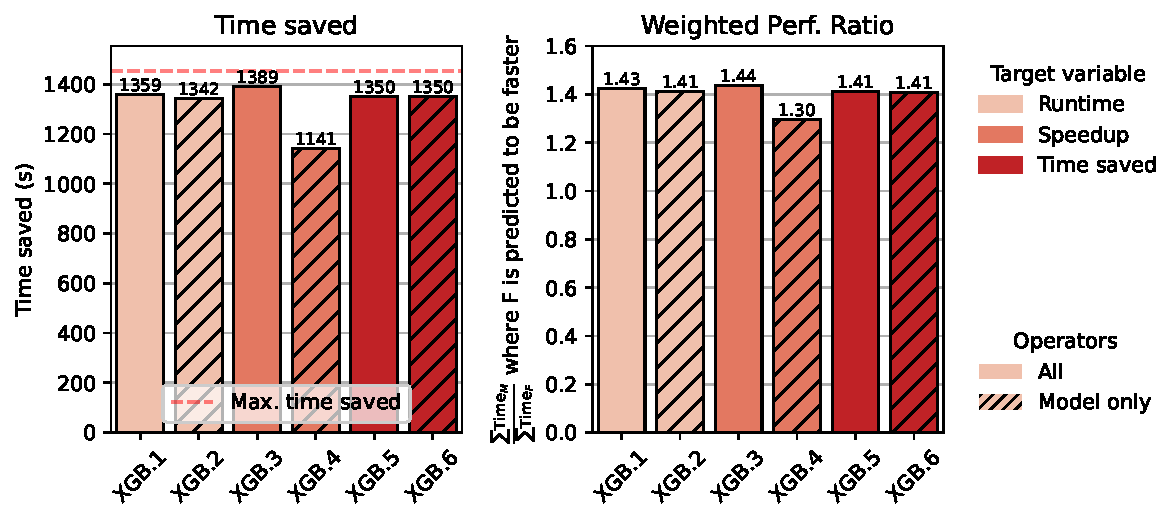
\includegraphics[width=\linewidth]{chapters/05_cost_estimation/figures/xgb-models-compare.pdf}
    \caption[XGBoost Estimator Comparison]{Evaluation of the XGBoost models on the validation set.}
    \label{fig:5-xgboost-evaluation}
\end{figure}

A comparative evaluation of the XGB models is shown in \autoref{fig:5-xgboost-evaluation}. As expected, these models, being more complex, outperform the linear regression models. Among the XGB models, there is minimal variation in performance on the validation set. There are no significant differences in performance based on the target variable used or whether all operators are included in the training set. XGB.3, which predicts the speedup of factorization over materialization, marginally surpasses the other models, accurately predicting 98\% of the validation scenarios.

\subsection{Comparing Performance}
\label{subsec:5-comparing-performance}
The performance of the two most effective estimators for each type is illustrated in \autoref{fig:5-model-cpu-gpu}. We plot the total time saved on the test scenarios, which includes the scenarios on the Hamlet and TPCx-AI datasets. As anticipated, the most complex and least explainable XGBoost models perform the best. Specifically, XGB.3 and XGB.5 save $600$ and $700$ seconds, respectively, of the total $1670$ seconds. The linear regression model performs the worst, likely due to overfitting to the synthetic data in the training set.

Interestingly, when we dissect the performance by compute type, the XGBoost models perform significantly better on GPU scenarios than on CPU scenarios, whereas LINR.5 performs better on CPU scenarios. This can be attributed to the fact that LINR.5 comprises two separate regressors, one for CPU and one for GPU, which enables it to capture the differences in the relationships between independent variables and runtime for each compute type. The process of combining these models to create a more accurate hybrid model is discussed in the following section.

\begin{figure}[ht]
    \centering
    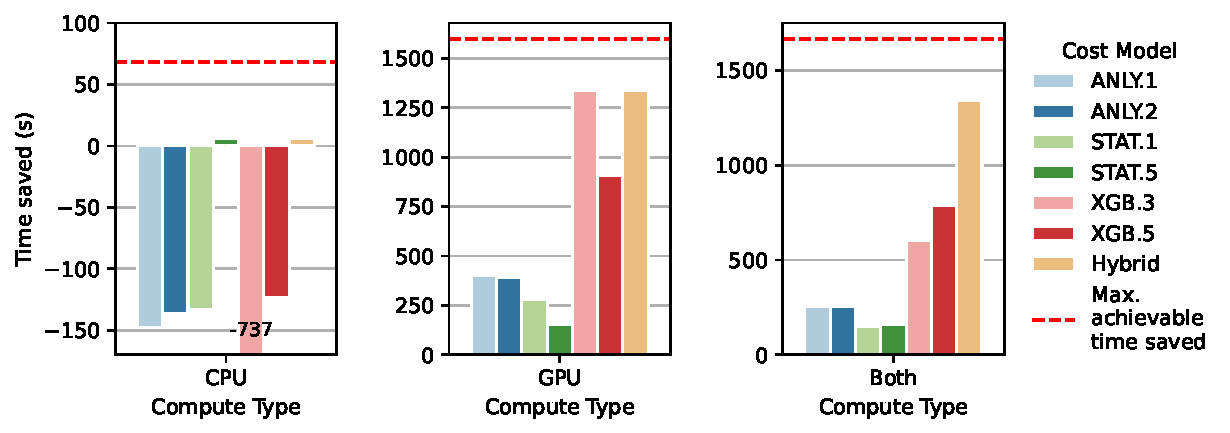
\includegraphics[width=0.9\linewidth]{chapters/05_cost_estimation/figures/compare_gpu_vs_cpu.pdf}
    \caption[Cost Model Comparison Broken Down by Compute Type]{Comparison of the best models, broken down by compute type. Evaluated on the test set.}
    \label{fig:5-model-cpu-gpu}
\end{figure}

\subsubsection{Combining Cost Models}
\label{subsec:5-hybrid}
To create the final cost model we combine the best of the models. We use the XGBoost model for GPU scenarios, and the LINR.5 model for CPU scenarios. This is done to capture the differences in the relationships between independent variables and runtime for each compute type. The final model is evaluated on the test set, and the results are shown in \autoref{fig:5-model-cpu-gpu}. The model achieves 80\% of the performance of a perfect cost model, saving 1344 seconds of the total 1670 seconds. This is a significant improvement over the best individual models, which achieved a maximum of 47\% of theoretical performance.

In order to construct the final cost model, we combine the best-performing models. We employ the XGB.3 model for GPU scenarios and the LINR.5 model for CPU scenarios. This approach is adopted to capture the differences in the relationships between independent variables and runtime for each compute type. The final model is evaluated on the test set, and the results are presented in \autoref{fig:5-model-cpu-gpu}. The model achieves $80\%$ of the performance of an ideal cost model, saving $1344$ seconds out of the total $1670$ seconds. This represents a significant improvement over the best individual models, which achieved a maximum of $47\%$ of theoretical performance.

\subsubsection{Meta-results}
In the Machine Learning (ML) framework proposed in \cite{amalur}, for which this thesis develops a cost model, the decision between factorization and materialization is made at runtime. Consequently, this should not introduce any overhead to the training process. We briefly touch upon the overhead introduced by the cost of inference of the models, as well as other factors that could influence the choice between cost models. An overview of all aspects is presented in \autoref{tab:5-meta-results}.

The first aspect that we examine is training time. For linear regression models, this is fast, but it is slower for the XGBoost model. The outliers in this case are the analytical models. ANLY.1 is notably slow as it necessitates fitting a large set of regressors, one for each combination of operator and F/M. On the contrary, ANLY.2 does not have a traditional training time as it employs a handcrafted formula.

In terms of extensibility, the ANLY.1 models are the easiest to extend for new ML models, as they already possess an inherent ``understanding'' of the used operators, provided by the included profiling metrics on LA operators. For the remaining models, an updated training set, which includes the new ML models, is required.

Arguably, the most crucial factor, other than performance, is inference speed, as we aim to avoid overhead in the training process. ANLY.2 and the linear regression model are very quick as they are simple equations with no more than $30$ terms. XGBoost, and consequently the hybrid model, is slightly slower but still fast. ANLY.1 is the slowest here, as computing the $OperatorCost$ of all involved operators is costly.

The final aspect is performance, which was discussed in the previous section.

\begin{table}[ht]
    \centering
    \begin{tabular}{lllll}
        \toprule
        Model             & Training time & Extensibility & Inference Speed & Performance \\
        \midrule
        Analytical 1      & Slow          & Easy          & Slow            & Bad         \\
        Analytical 2      & --            & Easy          & Quick           & Bad         \\
        Linear Regression & Fast          & Difficult     & Quick           & Bad         \\
        XGBoost           & Medium        & Difficult     & Medium          & Mediocre    \\
        Hybrid            & Medium        & Difficult     & Medium          & Good        \\
        \bottomrule
    \end{tabular}
    \caption{Qualitative comparison of the different models.}
    \label{tab:5-meta-results}
\end{table}

\subsection{Evaluating Feature Importance}
\label{subsec:6-feature-importance}
To determine which characteristics are most influential in the factorization/materialization (F/M) trade-off, we examine the final hybrid model, with a particular focus on the gain per feature from the GPU leg of the model.

We present the gain of the ten most influential features of the XGBoost model in \autoref{fig:5-gpu-feature-importance}. The gain quantifies the impact of a feature based on its contribution to reducing training error in the underlying decision trees. It can be interpreted as a measure of the influence a feature exerts on the model's prediction, which is insightful, as we are interested in identifying which features most significantly impact the F/M trade-off.
\begin{figure}[ht]
    \centering
    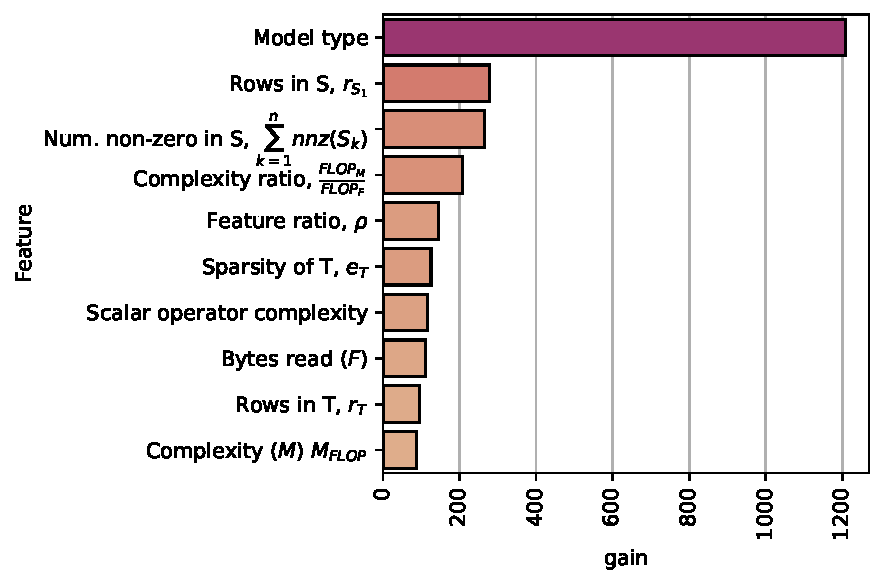
\includegraphics[width=0.75\linewidth]{chapters/05_cost_estimation/figures/xgboost-feat-importance.pdf}
    \caption[Feature importances of the hybrid model]{Feature importances of the Hybrid model, XGBoost (GPU) leg.}
    \label{fig:5-gpu-feature-importance}
\end{figure}

From the figure, we can deduce that the model type is the most impactful. This aligns with the results shown in \autoref{sec:5-motivation}, where we demonstrate that the choice of model significantly influences the F/M trade-off. Due to the operators used in each model, the speedup varies considerably between models, even when applied to the same dataset. For instance, factorized Gaussian training is beneficial twice as often compared to factorized KMeans. Other important features include data characteristics such as the number of rows in the tables ($r_{S_1}, r_T$), features related to the number of zeros in a table ($e_T, nnz(S)$), or features related to the differences between the materialized and factorized case ($\rho, \frac{FLOP_M}{FLOP_F}$). We observe that although the relationship between complexity and speedup was not as clear in \autoref{sec:5-motivation}, features related to the number of operations are important, even when considering only GPUs. This is evident from the relatively high gain of the materialized and scalar complexity. This is logical, as scalar operations have high speed-ups compared to other operators.

From these gain values we can conclude that, in our experiments, differences between GPUs are less impactful than differences in data characteristics and models. The GPU characteristic with the highest gain is a categorical feature for the GPU architecture, with a gain of $7$, followed by the L1 cache size and the number of Streaming Multiprocessors with gain values of $2.5$ and $1.4$, respectively.


